\documentclass[dvipdfmx]{jsarticle}
\usepackage[T1]{fontenc}
\usepackage[dvipdfmx]{hyperref}
\usepackage{lmodern}
\usepackage{latexsym}
\usepackage{amsfonts}
\usepackage{amssymb}
\usepackage{mathtools}
\usepackage{amsthm}
\usepackage{multirow}
\usepackage{graphicx}
\usepackage{wrapfig}
\usepackage{here}
\usepackage{float}
\usepackage{ascmac}
\usepackage{url}

\title{zoo.csvに関するR言語を使用した決定木構築}
\author{文理学部情報科学科\\5419045 高林 秀}
\date{\today}

\begin{document}

\maketitle

\begin{abstract}
  本稿では、今年度データ科学2で学習した「決定木構築手法」を使用して、本学部ページにて配布されたデータであるzoo.csvの決定木構築を実験するものである。また、決定木構築に際し、分割基準や木の高さなどのパラメータをいくつか変更しながら実験を行う。また得られた決定木の評価指標値として、精度の算出を行い、木の良し悪しを判定する。
\end{abstract}

\section{目的}
本稿では実際に、R言語を使用し配布データであるzoo.csvの決定木構築を行うことで、本年度データ科学2で学習した決定木構築の手法への理解を深め、その定着を図ることを目的とする。また、1年次に学習したlatexを用いたPDF作成の復習も兼ねるものとする。
\section{理論説明}
今回の実験で用いた、計算理論をそれぞれ説明する。
\subsection{分類学習について}
我々の生きている世界には様々なデータが存在する。例えば、農業を行う際「豊作になる条件」を知るには肥料の種類や量、光量や日照時間、温度、雨量等の様々な「属性の値」をもとに予測することが可能である。これを予測する手法として機械学習が挙げられるだろう。機械学習では、コンピュータがある問題とその答えを使用して学習を行い、データに潜むパターン等を識別、発見する技術である。この機械学習は大きく3つに系統が別れている。初めに「教師あり学習」、次に「教師なし学習」、最後に「強化学習」である。そしてそこから更に、求める結果や手法によって「分類」「回帰」「クラスタリング」「次元削減」「Q-Learning」と細かく分割される。中でも、今回扱う「分類」はデータが属するクラスを予測することを目的とする。予測するクラスが2つならば「2値分類」、それ以上ならば「多クラス分類」と呼ばれる。\par
詳細な説明は本稿では行わないが、今回扱う「決定木」は教師あり学習の分類に属する手法である。\par
これまで、分類の手法として「k-近傍法」等を学習してきた。k-近傍法は、最近傍のデータをk個選択し、それらが最も多く属するクラスに識別、分類を行う方法であった。決定木では、k-近傍法の手法とは異なり「木構造」を利用する。ある属性の属性値によってデータを徐々に分割していきクラス分類をする。決定木の詳細については後述する「決定木(Decision tree)」の部分で説明する。\par
なお分類学習には、ここで紹介した手法以外に「サポートベクターマシン(Support Vector Machine:通称SVM)」や 「ナイーブベイズ(Naive Bayes)」などがある。最近ではこれら従来の手法に加え、ニューラルネットワークを利用した手法が画像分類等の分野で広がっている(CNNなど)。
\begin{figure}[H]
  \centering
  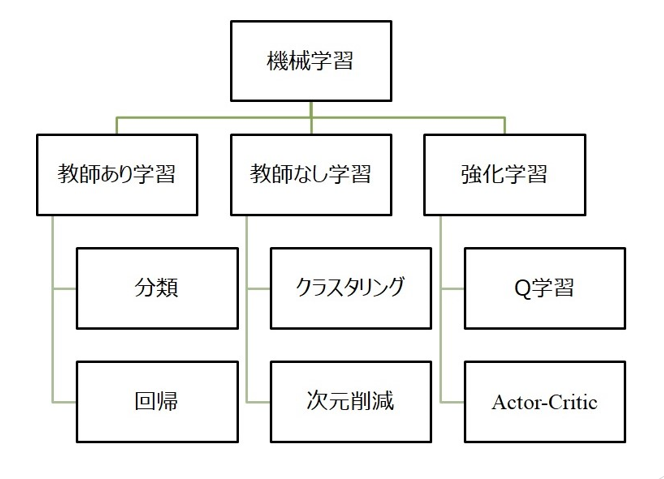
\includegraphics[scale=0.6]{ML.PNG}
  \caption{機械学習の枠組み}
\end{figure}
\subsection{決定木(Decision tree)}
決定木とは「木構造を利用した機械学習手法」である。分類を行う決定木を「分類木」、回帰(連続値の予測)を行う決定木は「回帰木」と呼ばれる。決定木では任意の属性の属性値による条件分岐によって、データを徐々に分割することで結果を出力する。したがって、生成される木構造の枝は分割の結果ラベルを、葉は予測、分類されるクラスの結果を、各ノードは属性に関する分割テスト含んでいる。\par
決定木を使用する例として、ミカンとリンゴを分類する場合を考える。下記の図のように、ミカンの画像を4枚、リンゴの画像を2枚の計6枚の画像データセットがあるとする。
これを、ある条件Aを定め、それに当てはまるもの、そうでないものを分割する。この操作を分割テストという。分割テストの結果によって次の分割テスト行うか否かが決定され、最終的に、ミカンとリンゴが図のように分類される。これが決定木の大まかな流れである。
\begin{figure}[H]
  \centering
  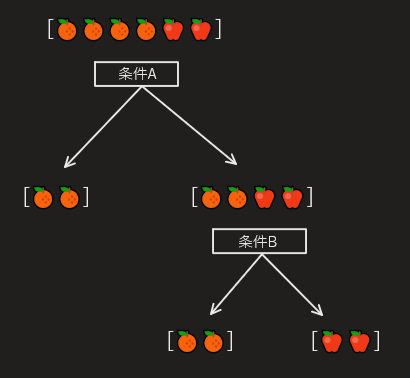
\includegraphics[scale=0.6]{decition_ex1.PNG}
  \caption{ミカンとリンゴの分類木}
\end{figure}
\subsubsection{決定木のメリット・デメリット}
決定木には、前項で述べたSVM等の他の機械学習手法よりも\textbf{分類課程が明確である}というメリットが存在する。これは、分類の結果の理由が他の手法よりも明確である点が挙げられるだろう。例えば先程のミカンとリンゴの例のように条件を満たすか否かによって、データを分割し、ミカンかリンゴか分類する。このとき何故ミカン(またはリンゴ)と分類したのかの理由が「条件A(または条件B)を満たしているから」と容易に説明できるであろう。\par
このように、機械学習を行った結果として生成されるモデルにおいて、判断の仕組みが分かる、説明できるものをホワイトボックス、反対に説明できないあるいは説明しづらいものをブラックボックスと呼ぶ。またホワイトボックスであるようなモデルを備えた人工知能を「説明可能なAI\footnote{説明可能なAI:このように、モデルの解釈性をもたらす研究が近年注目されており、ブラックボックス型のモデルを解釈する手法として「SHAP」「LIME」などがあり、Pythonパッケージが公開されるなど実務での利用が進んでいる。}(XAI:Explainable AI)」と呼ぶ。XAIは米国国防高等研究計画局(DARPA)が手動する研究プロジェクトが発端となった。\par
以下に、決定木のメリット・デメリットをまとめた表を示す。
\begin{table}[H]
  \begin{center}
    \caption{決定木のメリット・デメリット}
    \begin{tabular}{|c|c|} \hline
      メリット & デメリット \\ \hline
      ・学習結果の可読性が高く結果の根拠を説明しやすい & ・条件分岐が複雑になるほど過学習しやすい\\
      ・データの前処理が少なく済むことが多い & ・精度が突出して良いわけではない\\
      ・予測時に必要な計算量が小さい & \\
      ・回帰、分類の両方に対応可能 & \\ \hline
    \end{tabular}
    \label{hyo01}
  \end{center}
\end{table}
なお、下記サイトにおいて説明可能なAIの詳細な記載があるのでそのリンクを示す。\par
\url{https://blog.global.fujitsu.com/jp/2018-12-27/01/} \par
このように決定木は、分類課程が分かりやすいためエキスパートシステム\footnote{エキスパートシステム:ある分野における専門知識を蓄積し、その分野の専門家のように振る舞うことができる。}等に利用されることが多い。\par
決定木は、分割テストに使用する属性によって分割結果が変わることは、容易に想像することができる。データの属するクラスの割合をクラス分布と呼ぶ。決定木の分割テストでは、クラスを分類したいのでデータのクラス分布が偏れば偏るほど良い。しかし、分割テストに使用する属性によってクラス分布が偏ったり、均等になってしまいクラス分布があまり変化しない、といったことが発生する。そこで、分割テストに使用する属性を決定するためにいくつか評価基準が存在する。
\subsection{分割に用いる属性の選択基準}
分割テストに使用される属性は、下記のような評価基準を例に選出される。
\subsubsection{情報利得}
情報利得とは一言で言えば「クラスの偏りがどの程度進んだか」を表す数値である。データセット$D$のおける属性$A$の情報利得の計算式は下記。
\begin{center}
  \begin{align*}
    Gain_{A}(D) = H(D) - H_{A}(D) \\
  \end{align*}
\end{center}
この値が大きいほど、分割テストに適した良い属性ということになる。
\paragraph{情報量とエントロピー} \par
上記式の意味を説明するにあたって抑えておかなければならない概念がある。自己情報量(選択情報量)とエントロピー(平均情報量)である。\par
情報の数量的構造に関して甘利氏の著書「情報理論」\cite{amari01}に以下の記述があるので引用する。
\begin{quote}
  情報の数量的構造を論ずるにあたって、まず情報とは何であるかを考えなくてはなるまい。「(中略)」、すべての情報に共通な本質を抽象しよう。それは、「情報とはわれわれに何事かを教えてくれるものであり、われわれの不確実な知識を確実にしてくれるものである」というあたりまえのことである。「(中略)」。情報の量はその情報をもらったことによって知識の不確実さがどのくらい減ったかで計れば良いからである。
\end{quote}
すなわち、情報量とは、情報を得る前からその情報を得た後の差分で定義するということだ。
自己情報量とは下記式で表される数値である。
\begin{center}
  \begin{align*}
    -\log_2 p [bit]
  \end{align*}
\end{center}
これは、確率$p$の事象が発生したことを知らせる情報に含まれている情報量を示している。これが導かれるまでの課程は、甘利氏の著書「情報理論」\cite{amari01}の第1章「情報の数量的認識」の部分に記載があるのでそちらを参照いただきたい。この自己情報量は確率$p$が大きければ小さい値を取るという性質がある。言い換えれば、当たり前の事象が起こっても受け取れる情報は小さい、ということであり、これは、めったに起きない事象のほうが受け取る情報量が多いということを示している。\par
次に、エントロピーの説明をする。エントロピーとは平均情報量とも呼ばれる。これも、甘利氏の著書「情報理論」\cite{amari01}に記載があるので引用する。
\begin{quote}
  前項では、確率$p$の事象$A$が起こったときは、この情報量は$-\log_2 p$であることを論じた。「(中略)」。話をもう少し一般的にして$A_{1}, A_{2}, ..., A_{n}$の$n$個の事象があって、それぞれ$p_{1}, p_{2}, ..., p_{n}$の確率で生ずる場合を考えよう。
  \begin{center}
    \begin{align*}
        \Sigma_{i=1}^{n}p_{i} = 1
    \end{align*}
  \end{center}
  である。ここで、どの事象が起こったかを教えてもらうことにする。得られる情報の量は、どの$A$が生じたかで異なってくる。すなわち、$A_{1}$が起これば$-\log_2 p_{1}$、$A_{2}$ならば$-\log_2 p_{2}, ...$という情報が得られる。「(中略)」、得られる情報の量の期待値は$-\log_2 p_{i}$を確率$p_{i}$で平均したもの
  \begin{center}
    \begin{align*}
      I = -\Sigma_{i=1}^{n}p_{i}\log_2 p_{i}
    \end{align*}
  \end{center}
  である。
\end{quote}
これの$I$がエントロピーである。すなわち、自己情報量の平均(期待値)を表している。言い換えれば、どの$A_{i}$が起こったかを聞くときに得られる情報量である。
また、エントロピーについて甘利氏の著書「情報理論」\cite{amari01}では次のように記されている。
\begin{quote}
  われわれが情報をほしいのは、不確定な状況を確定したいからである。この場合、どういう情報がもらえるかは事前にわかるはずがなく、したがって、もらえる情報量そのものはわからない。わかるのはもらえる情報量の期待値だけである。この値は、不確定な状況を確定するのに要する平均情報量だといってもよい。
\end{quote}
すなわち、エントロピーとは「情報の不確定さ、程度」を表す数値である、ということだ。エントロピーの性質に関しては本稿では取り扱わないが、甘利氏の著書「情報理論」\cite{amari01}の第1章20ページに記載があるので、それを参照いただきたい。エントロピーは、クラス分布のばらつきが大きい時にエントロピーは値が小さくなり、分布が均等であるときには最大値1を取る性質がある。\par
ここまでの話を、先程の情報利得の話に当てはめてみる。このときの自己情報量を$I(c, D)|c:クラス, D:データセット(データ集合)$とすると、
\begin{center}
  \begin{align*}
    I(c, D) = -\log_2 P_{D}(c) \\
  \end{align*}
  ※$P_{D}(c)$:$D$中のデータのクラスが$c$となる確率
\end{center}
これは言い換えれば、確率$P_{D}(c)$で$D$のデータのクラスが$c$と分類されるときの情報量と捉えることができる。\par
そして、$D$を分割する前のエントロピーが$H(D)$で、属性$A$での分割後のエントロピーが$H_{A}(D)$であり、それぞれ下記式で示すことができる。
\newpage
\begin{center}
  \begin{align*}
    H(D)=\Sigma_{c \in C}P_{D}(c) \times I(c, D)=-\Sigma_{c \in C}P_{D}(c)\log_2 P_{D}(c) \\
  \end{align*}
  \begin{align*}
    H_{A}(D)=\Sigma_{a \in A}p_{D}(a) \times H(D_{a}) \\
  \end{align*}
  $P_{D}(a)$:$D$中のデータの属性$A$の属性値が$a$となる確率。
\end{center}
すなわち、クラス分布を偏らせるためには、情報利得が大きい属性を選択すれば良い。ここまでの話をまとめると、\textbf{情報利得 = 分割前のエントロピー - 分割後の各エントロピーの重み付き平均}ということになる。
\subsubsection{情報利得比}
情報利得には、分割数の大きい属性に対して、不当に高い値を返す問題がある。例として、ID番号(データの順番号)を分割属性に使用したとき、すべてのデータを別々の部分集合に分割することができるが、機械学習の目的である予測をするという意味において、全く役に立たない。そこで、分割数による正規化の必要性が生じる。そこで、新たな属性選択の評価基準として情報利得が挙げられる。\par
情報利得比とは、情報利得を分割情報量で正規化した数値である。
\paragraph{分割情報量}分割数が大きい属性に対して、より大きな値をとる性質を持つ。
\begin{center}
  \begin{align*}
    SI_{A}(D) = \Sigma_{a\in A}P_{D}(a) \times I(a, D) = \Sigma_{a\in A}P_{D}(a)\log_2 P_{D}(a)
  \end{align*}
\end{center}
情報利得比$GainRaito_{A}(D)$は下記式で計算される。
\begin{center}
  \begin{align*}
    GainRaito_{A}(D) = \frac{Gain_{A}(D)}{SI_{A}(D)}
  \end{align*}
\end{center}
\subsubsection{ジニ係数(Gini Index)}
分割後のデータ集合の、クラス分布が偏っている時、次の2つのことが言える。
\begin{itemize}
  \item その集合から取り出した2つの事例が同一のクラスに属する確率が高い。
  \item その集合から取り出した2つの事例が同一のクラスでない確率が低い。
\end{itemize}
この状況を利用した属性の評価基準がジニ係数である。ジニ係数では「2つの事例が同一のクラスでない確率」について考える。\par
前にも述べたように、決定木では、同一のクラスに属さない確率が低い方がクラスが偏っていて良いとされる。ここで、属性$A$に対するジニ係数を以下のように定める。
\begin{center}
  \begin{align*}
    Gini_{A}(D) = \Sigma_{a \in A}P_{D}(a) \times G(D_{a}) \\
    G(D) = 1 - \Sigma_{c \in C}P_{D}(c)^{2} \\
    P_{D}(c)^{2}:2事例があるクラスcに属する確率。
  \end{align*}
\end{center}
なお、ジニ係数は、集合から取り出した2つの事例が同一のクラスでない確率が低い、ということを表す数値なので、情報利得とは異なり、\textbf{より小さい値}の属性がよいとされる。
\subsection{決定木構築手法}
決定木の構築にあたって考慮しなければならないことがある。それはどのような木が望ましいかどうか、である。その際に以下2つの基準が存在する。
\begin{itemize}
  \item 木のコンパクトさ、単純さ
  \item 木の正確さ
\end{itemize}
すなわち望ましい木とは、「コンパクトかつ正確なもの」と言えるだろう。ここまで述べたように、決定木は分割に使用する属性によって木の構造が大きく変わる性質がある。したがって、最終的に形成される木の組み合わせは、非常に膨大な数になる。そのため、考えられるすべての木を計算し、評価するのには限界がある。よって、比較的計算量が少なく、簡単な方法で望ましい決定木を作る必要が生じる。この、簡単な方法で望ましい決定木を作る方法を「ヒューリスティックな方法」と呼ぶ。\par
決定木構築法の代表例としてTDIDT(Top Down Induction of Decision Trees)と呼ばれる手法が存在する。
\subsubsection{TDIDT}
ヒューリスティックに基づく決定木構築のアルゴリズムである。ここでいうTop Downとは、木の根から作るという意味で、Inductionとは、機能推論すなわちデータからモデルを構築する、という意味である。\par
TDIDTの大まかな流れは次の通り。
\begin{enumerate}
  \item 根となるデータ集合を用意する。
  \item ある基準(情報利得・情報利得比・ジニ係数)で属性を選ぶ。
  \item 選ばれた属性の属性値ごとにデータを分割する。
  \item 各枝に対して、3を繰り返す。
  \item 停止条件を満たす場合、その枝の分割を終了とする。
\end{enumerate}
上記の「停止条件」とは、これ以上データの分割ができない、あるいは、データを分割する必要がないと判定された場合のことである。では、具体的にどの様なときが停止条件に該当するのか説明する。
\paragraph{停止条件}
分類木の目的は「未知の事例」のクラスを予測することである。これを考慮した時、以下の場合が停止条件に該当する。
\begin{enumerate}
  \item すべての事例が同一クラスに属する時 \par
  予測するクラスが1つに定まるので、これ以上データを分割する必要がない。
  \item 分割する属性がない時 \par
  属性が離散属性、すなわちカテゴリである場合、一度分割テストで利用された属性は再度利用することができない。したがって、利用できる属性は徐々に減少していく。分割テストを繰り返す中で、データセットが持ち得る全属性を利用し尽くしてしまった場合、これ以上分割ができない。
  \item 分割の際、条件に合致する事例が少ない時 \par
  分類される事例数がある程度少なくなった場合、そこで分割テストを打ち切る。
  \item 分割に対して良い属性が見つからない時 \par
  すなわち、属性評価において、適切でないと判断された時、その属性で分割してもクラス分布がほとんど変化しないからである。前項でも述べたが、情報利得や情報利得比が小さい時若しくは、ジニ係数が大きい時に起こる。
\end{enumerate}
2,3において、最終的な事例の予測クラスは多数決で決定される。これをマジョリティクラスと呼ぶことがある。\par
このTDIDTをC言語での記述を模した疑似コードで表現すると以下のようになる。
※下記で記載している、A\_iやN\_iは数式で表現したときの$A_{i}, N_{i}$に相当する。
\begin{verbatim}
  void generate_decision_tree(N, DS, AL) {
      if(DSに含まれるデータがすべて同一クラスに属する) {
        そのクラスでNのラベル付を行う。
        Nをリーフノード(葉)とする。
        return 0;
      } else if(ALが空である) {
        if(DSの最も標準的なクラスである) {
          Nのラベル付を行う
          Nをリーフノードとする。
        return 0;
        }
      } else {
        最良属性を決定し、その最良属性の値でノードNをラベル付けする。
        for(int i = 0; i < 最良属性の値の種類の個数; i++) {
          最良属性の値A_iの分岐を作成する。
          その分岐を満たすデータ部分集合をS_iとする。
          分岐先のノードをN_iとする。
          if(S_iが空でない) {
            S_iを新たな入力サンプルデータとする。
            ALから最良属性を除いたものを新たな属性リストL_iとする。
            generate_decision_tree(N_i, S_i, L_i);
            決定木を分岐に接続する。
          } else {
            最も一般的なクラスでラベル付されたリーフノードを分岐に接続する。
          }
        }
      }
    }
\end{verbatim}
TDIDTはその特徴から、貪欲アルゴリズムと見なされることがある。\par
貪欲アルゴリズム(Greedy Search)とは、一般に「現在の状態を改善させる」という意味で、現時点で最善な方策を選択するアルゴリズムという意味で、山登り法や貪欲法などと呼ばれる。次の時点で最善の方策を選んだほうが、更に状態が良くなるだろうという可能性を考えず、その時点、現時点のみでの最善の方策を選択する。\par
TDIDTでは、前項で述べたジニ係数などの属性評価基準を使用して、分割テストで使用する属性を決定する。そしてその評価基準は、現在与えられた属性のみで分割したときの評価である。したがって、分割後のさらなる分割時の状態は考慮されていない。このことから、TDIDTは貪欲アルゴリズムであると言える。\par
加えて、TDIDTは分割統治法とも見なされることがある。\par
分割統治法(Divide and conquer)とは、一般に「問題全体をいくつかの小さな問題に分け、各部分の問題を解くことによって計算コスト(計算時間等)を減らそうとする手法」という意味である。\par
TDIDTでは、初めに選択された属性値にしたがってデータ集合をちいさな部分集合に分割する。次に、各部分集合に対して分割テストを行うことで決定木構築を目指す。すなわち、一つの大きな問題「データ集合」を複数の小さな問題「分割後の部分集合」に分けて、処理を進めているので、分割統治法であると言える。
\subsection{枝刈りと汎化性能(ロバスト性)}
機械学習全般の問題として「過学習」と呼ばれる問題が生じることがある。過学習とは、生成されたモデルが学習データに過剰に適合してしまう現状で、これにより未知のデータに対して正しい予測ができなくなってしまう。未知のデータに対する予測を行うのが本来の機械学習の目的であるはずなのにこれでは意味がない。決定木はもともと過学習が起こりにくい危害学習手法であるが、条件分岐が多くなりすぎる場合、すなわち木が複雑になりすぎると未知のデータに対する予測能力、汎化性能(ロバスト性)が低くなってしまう。この原因としては、学習データのノイズや外れ値によるもの、または、条件分岐でのルールの妥当性が低い等が考えられるだろう。\par
決定木において汎化性能を向上させる方法として「枝刈り」と呼ばれる手法が存在する。枝刈りは、過学習している枝、もしくは木を簡略化する手法である。これによって、木そのものが完結になり、分類精度の向上が見込まれる。枝刈りには、大きく分けて事前枝刈りと、事後枝刈りと呼ばれる方法が存在する。
\begin{itemize}
  \item 事前枝刈り\par
  該当する学習例が少ない場合、木の成長を止める手法である。これは、少ないデータに適合させようとすると過学習しやすくなってしまうためで、それを防ぐ目的がある、
  \item 事後枝刈り\par
  木が生成された後に、枝刈りを行う手法。事前枝刈りと比較して、枝刈りによる効果が大きい特徴を持つ。
  \begin{enumerate}
    \item 誤り削減枝刈り
    \item コスト複雑度枝刈り
    \item 悲観的枝刈り
  \end{enumerate}
  などといっいた手法が存在する。
\end{itemize}
\subsubsection{誤り削減枝刈り(reduced-error pruning)}
誤り削減枝刈りとは、決定木に対する誤り削減に基づいた枝刈りアルゴリズムである。\par
入力としては、学習済みの決定木と、検証用データを使用する。このアルゴリズムは枝刈り後の決定木を出力する。
\begin{enumerate}
  \item 決定木の根から遠い順に、木の各ノードに対して以下の操作を行う。
  \begin{enumerate}
    \item そのノード以下の部分木がカバーするデータを分割した際の正解率を計算する:accuraty
    \item そのノード以下の部分木がカバーするデータのマジョリティクラスを計算する:majoriry
    \item もし、accuraty $\leq$majoriryならば、その部分木をマジョリティクラスの葉に置き換える。
  \end{enumerate}
  \item 枝刈り後の決定木を出力する。
\end{enumerate}
つまり、エラー、誤りが減るときに部分木を葉で置換する。これによって精度の向上や、木を簡潔化することができる。すなわちコンパクトで正確な木が出来上がる。
\subsubsection{コスト複雑度枝刈り}
各ノードを根とする部分木の評価値を次のように定め、この評価値が閾値を超えた場合、枝刈りの対象とする手法である。
\begin{center}
  コスト評価関数=学習データによる部分木のエラーコスト+$\alpha \times$部分木の葉の数 \par
  $\alpha$:木の「簡潔さ」と「正確さ」どちらを重視するかを示す数値
\end{center}
一般に、木の「簡潔さ」と「正確さ」は相反する関係(トレードオフ)にある。つまり、木を簡潔にすればするほど正確さ(精度)は低くなるが、反対に正確さを上げれば、木はより複雑になる、ということである。\par
コスト評価関数は、「学習データを使用した見かけ上のエラーコスト」と「部分木の葉の数」の和、すなわち「不正確さ」と「複雑さ」の和を計算していると言って良い。したがって。コスト評価関数が』低ければ低いほど良い部分木であり、コスト評価関数の値が閾値を超えた場合というのは、その部分木が「不正確かつ複雑である」という意味になるので、枝刈りを行う。
\begin{center}
  $\tilde{T}:部分木Tに含まれる葉ノードの集合$
  \begin{align*}
    R_{\alpha}(T) = R(T) + \alpha|\tilde{T}|
  \end{align*}
  \begin{align*}
    R(T) = \Sigma_{t \in \tilde{T}}R(t) whereR(t) = \frac{M(t)}{N}\\
  \end{align*}
  \begin{align*}
    R(T):Tの誤り率\\
    M(t):ノードtにおける誤分類事例数\\
    N:データ数
  \end{align*}
\end{center}
評価値$R_{\alpha}$を最小にする$T$の部分木$T'$を求めたい。しかしこれは、一度では求めることはできない。したがって、徐々に近づけるように計算する。
\begin{center}
  $T_{t}:部分木Tにおいて、ノードtを根とする部分木$ \par
  $R_{\alpha}(t):T_{t}を葉に置き換えたときの評価値$ \par
  $R_{\alpha}(T_{t}):T_{t}の評価値$
  \begin{align*}
      R_{\alpha}(t) = R(t) + \alpha \leq R(T_{t})+\alpha|\tilde{T}|\\
      =R_{\alpha}(T_{t})
  \end{align*}
\end{center}
上記式を変形すると下記式が得られる。
\begin{center}
  \begin{align}
    \frac{R(t)-R(T_{t})}{|\tilde{T}-1|} \leq \alpha
  \end{align}
\end{center}
すなわち、左辺を最小にする$t$を葉に置き換える動作を繰り返すことで、目的の決定木へ近づけていく。
\subsubsection{悲観的枝刈り}
前項で述べた「誤り削減枝刈り」では評価用のデータを必要とした。この悲観的枝刈りでは、学習データをサンプルと見なすことで評価用のデータを不要にした枝刈り手法である。\par
葉ノードに含まれる$n$個のデータを母集団から取り出し、標本とする。その標本のエラー率から母集団のエラー率を統計的に推定し、推定したエラー率によって枝刈りを行う。\par
誤り削減枝刈りと、悲観的枝刈りに共通する点として「エラー率pが小さくなる場合に決定木を決めるという点が挙げられる。両者の違いとして、「エラー率の計算方法」がある。誤り削減枝刈りでは、評価用データを利用してエラー律を計算したが、悲観的枝刈りでは、学習データと標本と母集団の統計的推定を使用してエラー率を計算している。
\subsection{決定木の評価指標}
機械学習で生成されたモデルには当然、その良し悪しを評価する必要がある。機械学習の目的は未知のデータに対する予測である。したがって未知データに対する適合性を高める必要が生じるが、手元に存在しないデータを学習に利用することはできない。したがって、機械学習ではデータの一部分を検証用データとして正解を隠した状態にすることで擬似的に未知データを作り、性能を評価する、といったことが行われる。この擬似的に未知のデータを得る方法として、ホールドアウト法(Hold Out)や交差検証法(Cross Validation)が存在する。\par
\paragraph{ホールドアウト法}\par
ホールドアウト法では、手元に存在するデータセットを、モデルの構築に使用する「学習データ(教師データ)」と「検証用データ」に分割して利用する手法である。このとき、検証用データを学習に利用しないことで評価時に、未知データとして利用することが可能となる。
\begin{figure}[H]
  \centering
  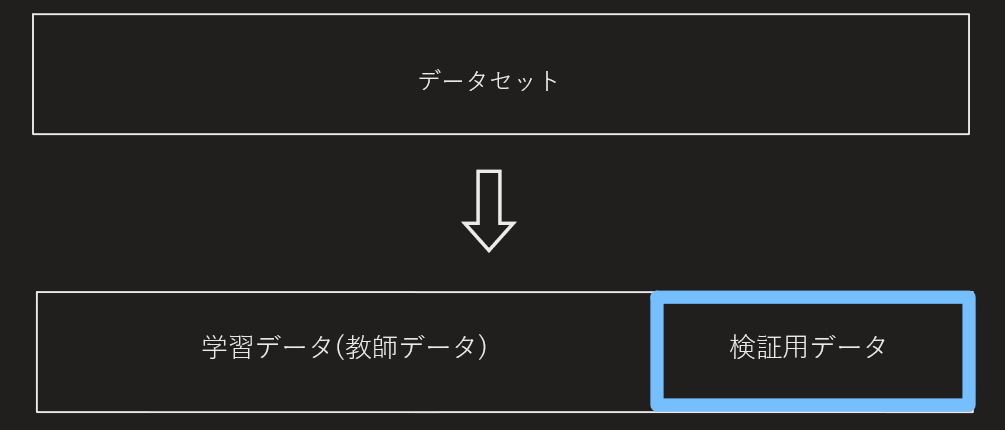
\includegraphics[scale=0.3]{HoldOut.PNG}
  \caption{ホールドアウト法}
\end{figure}
\paragraph{交差検証法}\par
ホールドアウト法は、シンプルで非常に分かりやすい手法だが、評価データが偶然モデルに適合し高い評価値を示してしまう場合があるという欠点を抱えている。すなわち1回検証するだけでは、そのデータがたまたまモデルに適合したデータである可能性があり、実際には過学習が起きているのに、良い評価値を出力してしまう、ということだ。\par
交差検証法では、上記に述べた欠点を回避するために、複数回、異なるデータで検証を行う。まず手元にあるデータセットを任意の数$k$で分割する。このうち1つを検証用データとして、残りを学習データとして使用する。次に、先程使用した検証用データとは別のデータを次の評価時に使用する。これを$k$回繰り返す。最終的な評価値は、各回の評価値の平均を利用する。
\begin{figure}[H]
  \centering
  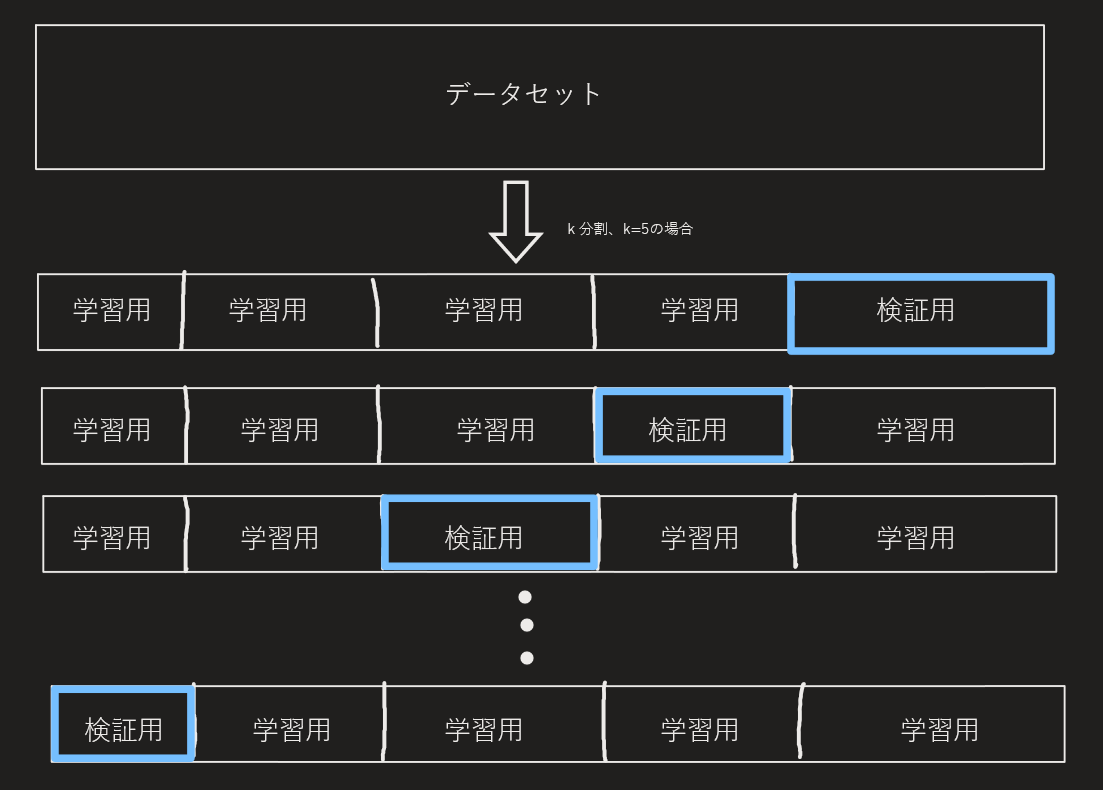
\includegraphics[scale=0.3]{cross.PNG}
  \caption{交差検証法}
\end{figure}
なお、評価値を決める評価指標は次のものが挙げられる。
\begin{itemize}
  \item 精度(accuracy)
  \item 分割表(混同行列)による解析
  \item 統計的推定
\end{itemize}
などがある。
\subsubsection{精度}
決定木における最も単純で、基本的な評価指標である。単純に、「予測が正解したテスト例の数」をテスト例の総数で割った値を利用する。すなわち、どれだけ正確な予測ができたか、をすぐに知ることができる指標と言える。
\begin{center}
  \begin{align*}
    精度accuracy = \frac{正解したテスト数}{テストの総数}
  \end{align*}
\end{center}
\subsubsection{分割表による評価}
なお、決定木の評価指標は上記に挙げた精度以外に、再現率、適合率、F値などがある。このとき、例として「陽性、陰性」の2値分類を考える。この分類において、結果と予測の組み合わせは$2\times4$行列となる。
\begin{table}[H]
  \begin{center}
    \caption{混同行列}
    \begin{tabular}{|l|l|l|} \hline
      実際の値/予測値 & 陽性(Positive) & 陰性(Negative) \\ \hline
      陽性(Positive) & 真陽性(True Positive) & 偽陰性(False Negative)\\ \hline
      陰性(Negative) & 偽陽性(False Positive) & 真陰性(True Negative) \\ \hline
    \end{tabular}
    \label{hyo02}
  \end{center}
\end{table}
上記の組み合わせを「混同行列」または「分割表」と呼ぶ。
\paragraph{再現率(recall)}\par

\paragraph{適合率(precision)}
\paragraph{F値(F-Measure)}



\paragraph{paragraph name}

\subsubsection{交差検定}




\section{計算機実験}
\subsection{実験準備}
  \subsubsection{実験環境}
  今回の実験は仮想マシン上でR言語を起動し行った。下記に実験時の環境を示す。
  \begin{itemize}
    \item ホストOS:Window10 Home Ver.20H2
    \item 仮想OS:Ubuntu 20.04.2 LTS
    \item CPU:Intel(R)Core(TM)i7-9700K @ 3.6GHz
    \item GPU:Nvidia Geforce RTX2070 OC @ 8GB
    \item ホストRAM:16GB
    \item 仮想RAM:4GB
  \end{itemize}
\subsubsection{実験データ}
\subsubsection{実験結果}
\subsubsection{結果の説明}
\section{考察}
\section{まとめ}
\begin{thebibliography}{99}
  \bibitem {amari01} 甘利俊一、『情報理論』、ちくま文庫、2011年4月10日
\end{thebibliography}
\end{document}
